% LINGI2252 - Measures & Maintenance
% Code Analysis
\documentclass[12pt, a4paper]{article}
\usepackage[utf8]{inputenc}
\usepackage[UKenglish]{babel}
\usepackage{graphicx}				% Use pdf, png, jpg, or eps§ with pdflatex; use eps in DVI mode
\usepackage{xcolor}
\usepackage{listings}
\usepackage{hyperref}
\usepackage{tabularx}
\usepackage{array}
\usepackage{longtable}
\usepackage{multirow}
\usepackage[babel=true]{csquotes}

\usepackage[T1]{fontenc}

\lstset{%
	basicstyle=\ttfamily\small,
	commentstyle=\color{green!90!black},
	frame=single,
	keywordstyle=\bfseries\color{blue},
	language=python,
	numberstyle=\color{gray},
%	tabsize=2,
}


\hypersetup{%
	colorlinks=true,
	linkcolor=blue,
	urlcolor=blue
}


\newcommand{\tbf}[1]{\textbf{#1}}
\newcommand{\tit}[1]{\textit{#1}}
\newcommand{\ttt}[1]{\texttt{#1}}

\newcommand{\noi}{\noindent}

\newcommand{\pyl}{\textsf{Pylint}}

% Error messages
% ---------------------
% C
\newcommand{\Cztwzth}{Metaclass method \%s should have \tit{mcs} as first argument}
\newcommand{\Czthtwo}{More than one statement on a single line}
\newcommand{\Czthtwf}{Comma not followed by a space}
% E
\newcommand{\Ezozo}{Explicit return in \_\_init\_\_}
\newcommand{\Eztwzth}{Access to member \%r before its definition line \%s}
\newcommand{\Eztwoo}{Method has no argument}
\newcommand{\Ezseoz}{Raising a new style class which doesn't inherit from BaseException}
\newcommand{\Eozztw}{Use of super on an old style class}
% R
\newcommand{\Rznoo}{Too many return statements (\%s/\%s)}
\newcommand{\Rznotw}{Too many branches (\%s/\%s)}
\newcommand{\Rznoth}{Too many arguments (\%s/\%s)}
\newcommand{\Rznof}{Too many local variables (\%s/\%s)}
% W
\newcommand{\Wzoztw}{Dangerous default value \%s as argument}
\newcommand{\Wztwzo}{Attribute \%r defined outside \_\_init\_\_}
\newcommand{\Wztwtwo}{Arguments number differs from \%s method}
\newcommand{\Wztwtho}{\_\_init\_\_ method from base class \%r is not called}
\newcommand{\Wztwthtw}{Class has no \_\_init\_\_ method}
\newcommand{\Wztwthth}{\_\_init\_\_ method from a non direct base class \%r is called}
\newcommand{\Wzfzth}{Relative import \%r, should be \%r}
\newcommand{\Wzfzf}{Reimport \%r (imported line \%s)}
\newcommand{\Wzsztw}{Using global for \%r but no assignment is done}
\newcommand{\Wzsotw}{Unused variable \%r}
\newcommand{\Wzstwo}{Redefining name \%r from outer scope (line \%s)}
\newcommand{\Wzstwtw}{Redefining built-in \%r}
\newcommand{\Wzstho}{Using possibly undefined loop variable \%r}
\newcommand{\Wzseztw}{No exception type(s) specified}
\newcommand{\Wzsezth}{Catching too general exception \%s}


\newcommand{\mytab}[5]{
	\begin{tabularx}{\textwidth}{|c|X|}
	\hline
	\tbf{Correlation}		& #1 \\
	\hline
	#2	& #3 \\
	\hline
	#4	& #5 \\
	\hline
	\end{tabularx}
}



\def\blurb{\textsc{Université catholique de Louvain\\
  École polytechnique de Louvain\\
  Pôle d'ingénierie informatique}}
\def\clap#1{\hbox to 0pt{\hss #1\hss}}%
\def\ligne#1{%
  \hbox to \hsize{%
    \vbox{\centering #1}}}%
\def\haut#1#2#3{%
  \hbox to \hsize{%
    \rlap{\vtop{\raggedright #1}}%
    \hss
    \clap{\vbox{\vfill\centering #2\vfill}}%
    \hss
    \llap{\vtop{\raggedleft #3}}}}%
\begin{document}

\begin{titlepage}
\thispagestyle{empty}\vbox to 1\vsize{%
  \vss
  \vbox to 1\vsize{%
    \haut{\raisebox{-2mm}{
\includegraphics[width=2.5cm]{logo_epl.jpg}}}{\blurb}{\raisebox{-5mm}{
\includegraphics[scale=0.20]{ingi_logo.png}}}
    \vfill
    \ligne{\Huge \textbf{\textsc{LINGI2252}}}
     \vspace{5mm}
    \ligne{\huge \textbf{\textsc{Software Engineering : measures and maintenance}}}
     \vspace{15mm}
    \ligne{\Large \textbf{\textsc{Assignment step 4: \\Study patterns of co-occurring code improvements}}}
    \vspace{5mm}
    \ligne{\large{\textsc{\today}}}
    \vfill
    \vspace{5mm}
    \ligne{%
         \textsc{Professor\\Kim Mens}
      }
      \vspace{10mm}
    }%
    \ligne{%
         \textsc{Group 23\\Michael Heraly\\Thibault Gerondal}
      }
      \vspace{5mm}
  \vss
  }
\end{titlepage}






\section{Introduction}

In our previous reports, we analyzed Reddit with \pyl{}.
We first learned how to use \pyl{} and analyzed the messages that it can deliver.
Then, we analyzed all the messages given by \pyl{} for Reddit to see if they are relevant and concise.\\

In this report, we will study the links that can exist between the different error codes that \pyl{} gives for the Reddit project.
This will allow us to assess if the \pyl{} messages are redundant.


\section{Methodology}

We parsed the \pyl{} output with a home-made script to generate a table containing the correlations between the different error codes.
We made three tables for three levels of analysis : by file, by class, and by method.
\pyl{} generates error messages, and sometimes specify the class and the method concerned.
For the file-level, we considered the messages where no class was specified.
For the class-level, we only selected the messages where \pyl{} indicates a class.
And for the method-level, we only considered the messages where \pyl{} indicates a method.

\bigskip
To refine our analysis, we removed some error codes that weren't relevant for the analysis.
We discarded pairs of error codes that had high distances (greater than 0.9).
And we excluded all pairs of critics for which one of the code-critics covers more than 90\% of all source code entities analyzed.

\bigskip
The report tables are in the Appendices section.
In the tables, we only displayed the values of the correlations that were lower than 90\%.
We did not display correlation with value 0.
There is also a color scale to make values more visible.

\bigskip
In our analysis, we only focused our attention to the pair of codes that had a correlation lower than 70\%, because correlations with higher values have less impact.



\section{Patterns of Co-occurring Critics}

\subsection{By file}

\subsubsection*{Unfortunate Correlation}

This section contains pairs of error codes that have quite a low distance, but the error codes don't have something in common.

\bigskip \noi
\begin{tabularx}{\textwidth}{|c|X|}
\hline
\tbf{Correlation}		& 0.50 \\
\hline
C0322		& Operator not preceded by a space \\
\hline
R0904		& Too many public methods (\%s/\%s) \\
\hline
\end{tabularx}

\bigskip \noi
\begin{tabularx}{\textwidth}{|c|X|}
\hline
\tbf{Correlation}		& 0.67 \\
\hline
C0322		& Operator not preceded by a space \\
\hline
R0911		& Too many return statements (\%s/\%s) \\
\hline
\end{tabularx}


\bigskip \noi
\begin{tabularx}{\textwidth}{|c|X|}
\hline
\tbf{Correlation}		& 0.50 \\
\hline
C0322		& Operator not preceded by a space \\
\hline
R0912		& Too many branches (\%s/\%s) \\
\hline
\end{tabularx}


\bigskip \noi
\begin{tabularx}{\textwidth}{|c|X|}
\hline
\tbf{Correlation}		& 0.50 \\
\hline
C0322		& Operator not preceded by a space \\
\hline
W0106		& Expression "\%s" is assigned to nothing \\
\hline
\end{tabularx}


\bigskip \noi
\begin{tabularx}{\textwidth}{|c|X|}
\hline
\tbf{Correlation}		& 0.50 \\
\hline
C0322		& Operator not preceded by a space \\
\hline
W0404		& Reimport \%r (imported line \%s) \\
\hline
\end{tabularx}


\bigskip \noi
\begin{tabularx}{\textwidth}{|c|X|}
\hline
\tbf{Correlation}		& 0.67 \\
\hline
C0322		& Operator not preceded by a space \\
\hline
W0631		& Using possibly undefined loop variable \%r \\
\hline
\end{tabularx}

\bigskip \noi
\begin{tabularx}{\textwidth}{|c|X|}
\hline
\tbf{Correlation}   & 0.60 \\
\hline
E0611   & No name \%r in module \%r \\
\hline
W0232   & Class has no \_\_init\_\_ method \\
\hline
\end{tabularx}

\bigskip \noi
\begin{tabularx}{\textwidth}{|c|X|}
\hline
\tbf{Correlation}   & 0.70 \\
\hline
E1101   & \%s \%r has no \%r member \\
\hline
R0914   & Too many local variables (\%s/\%s) \\
\hline
\end{tabularx}

\bigskip \noi
\begin{tabularx}{\textwidth}{|c|X|}
\hline
\tbf{Correlation}   & 0.50 \\
\hline
R0911   & Too many return statements (\%s/\%s) \\
\hline
R0912   & Too many branches (\%s/\%s) \\
\hline
Comment: & \textit{In Reddit, they use a lot of if/return.} \\
\hline
\end{tabularx}

\bigskip \noi
\begin{tabularx}{\textwidth}{|c|X|}
\hline
\tbf{Correlation}   & 0.67 \\
\hline
R0911   & Too many return statements (\%s/\%s) \\
\hline
W0631   & Using possibly undefined loop variable \%r \\
\hline
\end{tabularx}

\bigskip \noi
\begin{tabularx}{\textwidth}{|c|X|}
\hline
\tbf{Correlation}   & 0.50 \\
\hline
R0912   & Too many branches (\%s/\%s) \\
\hline
W0631   & Using possibly undefined loop variable \%r \\
\hline
\end{tabularx}

\bigskip \noi
\begin{tabularx}{\textwidth}{|c|X|}
\hline
\tbf{Correlation}   & 0.50 \\
\hline
W0404   & Reimport \%r (imported line \%s) \\
\hline
W0631   & Using possibly undefined loop variable \%r \\
\hline
\end{tabularx}

% end unfortunate correlation

\subsubsection*{Same niche}
This occurs when code critics seem to correlate just because they both refer to a specific kind of source entity.

\bigskip \noi
\begin{tabularx}{\textwidth}{|c|X|}
\hline
\tbf{Correlation}   & 0.50 \\
\hline
R0911   & Too many return statements (\%s/\%s) \\
\hline
R0912   & Too many branches (\%s/\%s) \\
\hline
Comment: & \textit{In Reddit, they use a lot of if/return in series.}\\
\hline
\end{tabularx}


\bigskip \noi
\begin{tabularx}{\textwidth}{|c|X|}
\hline
\tbf{Correlation}   & 0.68 \\
\hline
R0913   & Too many arguments (\%s/\%s) \\
\hline
R0914   & Too many local variables (\%s/\%s) \\
\hline
Comment: & \textit{When declaring arguments, you usually create a local variable to manipulate the data.}\\
\hline
\end{tabularx}

\bigskip \noi
\begin{tabularx}{\textwidth}{|c|X|}
\hline
\tbf{Correlation}   & 0.67 \\
\hline
R0914   & Too many local variables (\%s/\%s) \\
\hline
W0612   & Unused variable \%r \\
\hline
Comment: & \textit{Declaring useless variables will have an impact on the number of local variables.}\\
\hline
\end{tabularx}

\bigskip \noi
\begin{tabularx}{\textwidth}{|c|X|}
\hline
\tbf{Correlation}   & 0.69 \\
\hline
W0612   & Unused variable \%r \\
\hline
W0621   & Redefining name \%r from outer scope (line \%s) \\
\hline
Comment: & \textit{Maybe the variable was not that useless !}\\
\hline
\end{tabularx}

% end same nich


\bigskip
\subsection{By class}

\subsubsection*{Unfortunate Correlation}
This section contains pairs of error codes that have quite a low distance, but the error codes don't have something in common.

\bigskip \noi
\mytab{0.50}{C0203}{\Cztwzth{}}{E0101}{\Ezozo{}}

\bigskip \noi
\mytab{0.50}{C0203}{\Cztwzth{}}{W0231}{\Wztwtho{}}

\bigskip \noi
\mytab{0.50}{C0203}{\Cztwzth{}}{W0631}{\Wzstho{}}

\bigskip \noi
\begin{tabularx}{\textwidth}{|c|X|}
\hline
\tbf{Correlation}   & 0.67 \\
\hline
C0203   & \Cztwzth{} \\
\hline
W0233   & \Wztwthth{} \\
\hline
\end{tabularx}

\bigskip \noi
\mytab{0.67}{C0203}{\Cztwzth{}}{W0702}{\Wzseztw{}}

\bigskip \noi
\mytab{0.67}{C0203}{\Cztwzth{}}{W0703}{\Wzsezth{}}

\bigskip \noi
\mytab{0.67}{E0101}{\Ezozo{}}{R0912}{\Rznotw{}}

\bigskip \noi
\mytab{0.67}{E0101}{\Ezozo{}}{W0403}{\Wzfzth{}}

\bigskip \noi
\mytab{0.50}{E0101}{\Ezozo{}}{W0702}{\Wzseztw{}}

\bigskip \noi
\mytab{0.50}{E0101}{\Ezozo{}}{W0703}{\Wzsezth{}}

\bigskip \noi
\mytab{0.67}{E0203}{\Eztwzth{}}{R0912}{\Rznotw{}}

\hrule
\bigskip \noi
\mytab{0.67}{R0912}{\Rznotw{}}{W0231}{\Wztwtho{}}

\bigskip \noi
\mytab{0.50}{R0912}{\Rznotw{}}{W0403}{\Wzfzth{}}

\bigskip \noi
\mytab{0.60}{R0912}{\Rznotw{}}{W0404}{\Wzfzf{}}

\bigskip \noi
\mytab{0.67}{R0912}{\Rznotw{}}{W0602}{\Wzsztw{}}

\bigskip \noi
\mytab{0.67}{R0912}{\Rznotw{}}{W0631}{\Wzstho{}}

\bigskip \noi
\mytab{0.67}{W0231}{\Wztwtho{}}{W0403}{\Wzfzth{}}

\bigskip \noi
\mytab{0.50}{W0231}{\Wztwtho{}}{W0702}{\Wzseztw{}}

\bigskip \noi
\mytab{0.50}{W0231}{\Wztwtho{}}{W0703}{\Wzsezth{}}

\hrule
\bigskip \noi
\mytab{0.50}{W0233}{\Wztwthth{}}{W0602}{\Wzsztw{}}

\bigskip \noi
\mytab{0.50}{W0233}{\Wztwthth{}}{W0631}{\Wzstho{}}

\bigskip \noi
\mytab{0.67}{W0233}{\Wztwthth{}}{W0702}{\Wzseztw{}}

\bigskip \noi
\mytab{0.67}{W0233}{\Wztwthth{}}{W0703}{\Wzseztw{}}

\bigskip \noi
\mytab{0.60}{W0403}{\Wzfzth{}}{W0404}{\Wzfzf{}}

\bigskip \noi
\mytab{0.67}{W0403}{\Wzfzth{}}{W0602}{\Wzsztw{}}

\bigskip \noi
\mytab{0.67}{W0403}{\Wzfzth{}}{W0631}{\Wzstho{}}

\hrule
\bigskip \noi
\mytab{0.50}{W0602}{\Wzsztw{}}{W0702}{\Wzseztw{}}

\bigskip \noi
\mytab{0.50}{W0602}{\Wzsztw{}}{W0703}{\Wzsezth{}}

\hrule
\bigskip \noi
\mytab{0.50}{W0631}{\Wzstho{}}{W0702}{\Wzseztw{}}

\bigskip \noi
\mytab{0.50}{W0631}{\Wzstho{}}{W0703}{\Wzsezth{}}

\hrule
\bigskip \noi
\mytab{0.67}{W0702}{\Wzseztw{}}{W0703}{\Wzsezth{}}

% end unfortunate correlation

\subsubsection*{Same niche}
This occurs when code critics seem to correlate just because they both refer to a specific kind of source entity.

\bigskip \noi
\begin{tabularx}{\textwidth}{|c|X|}
\hline
\tbf{Correlation}   & 0.50 \\
\hline
E0101   & \Ezozo{} \\
\hline
W0233   & \Wztwthth{} \\
\hline
Comment: & \textit{It seems like they use a class to return something.. This is a bad practice that makes these messages correlated.}\\
\hline
\end{tabularx}

% end same nich

\subsection{By method}

\subsubsection*{Unfortunate Correlation}
This section contains pairs of error codes that have quite a low distance, but the error codes don't have something in common.

\bigskip \noi
\begin{tabularx}{\textwidth}{|c|X|}
\hline
\tbf{Correlation}   & 0.60 \\
\hline
C0203   &  Metaclass method \%s should have mcs as first argument \\
\hline
W0602   &  Using global for \%r but no assigment is done \\
\hline
\end{tabularx}


\bigskip \noi
\begin{tabularx}{\textwidth}{|c|X|}
\hline
\tbf{Correlation}   & 0.60 \\
\hline
F0401   &  Unable to import \%s \\
\hline
W0122   &  Use of exec \\
\hline
\end{tabularx}

\subsubsection*{Same niche}
This occurs when code critics seem to correlate just because they both refer to a specific kind of source entity.

\bigskip \noi
\begin{tabularx}{\textwidth}{|c|X|}
\hline
\tbf{Correlation}   & 0.81 \\
\hline
W0233   &  \_\_init\_\_ method from a non direct base class \%r is called \\
\hline
W0231   &  \_\_init\_\_ method from base class \%r is not called \\
\hline
Comment: & \textit{The source is the same. The \_\_init\_\_ is not called at the right location.}\\
\hline
\end{tabularx}


\bigskip

\section{Conclusion}

We analysed the \pyl{} messages for the Reddit project.
We found out that some error codes were correlated, but this was due to the fact that they refer to the same source entity.
It turns out that most of the correlations were unfortunate correlation.
\pyl{} is quite good, because we did not find error codes that were clearly correlated.



\newpage
\section*{Appendices}

\renewcommand{\textfraction}{0.01}
\renewcommand{\topfraction}{0.01}
\renewcommand{\bottomfraction}{0.01}
\renewcommand{\floatpagefraction}{0.01}
\setcounter{totalnumber}{1}

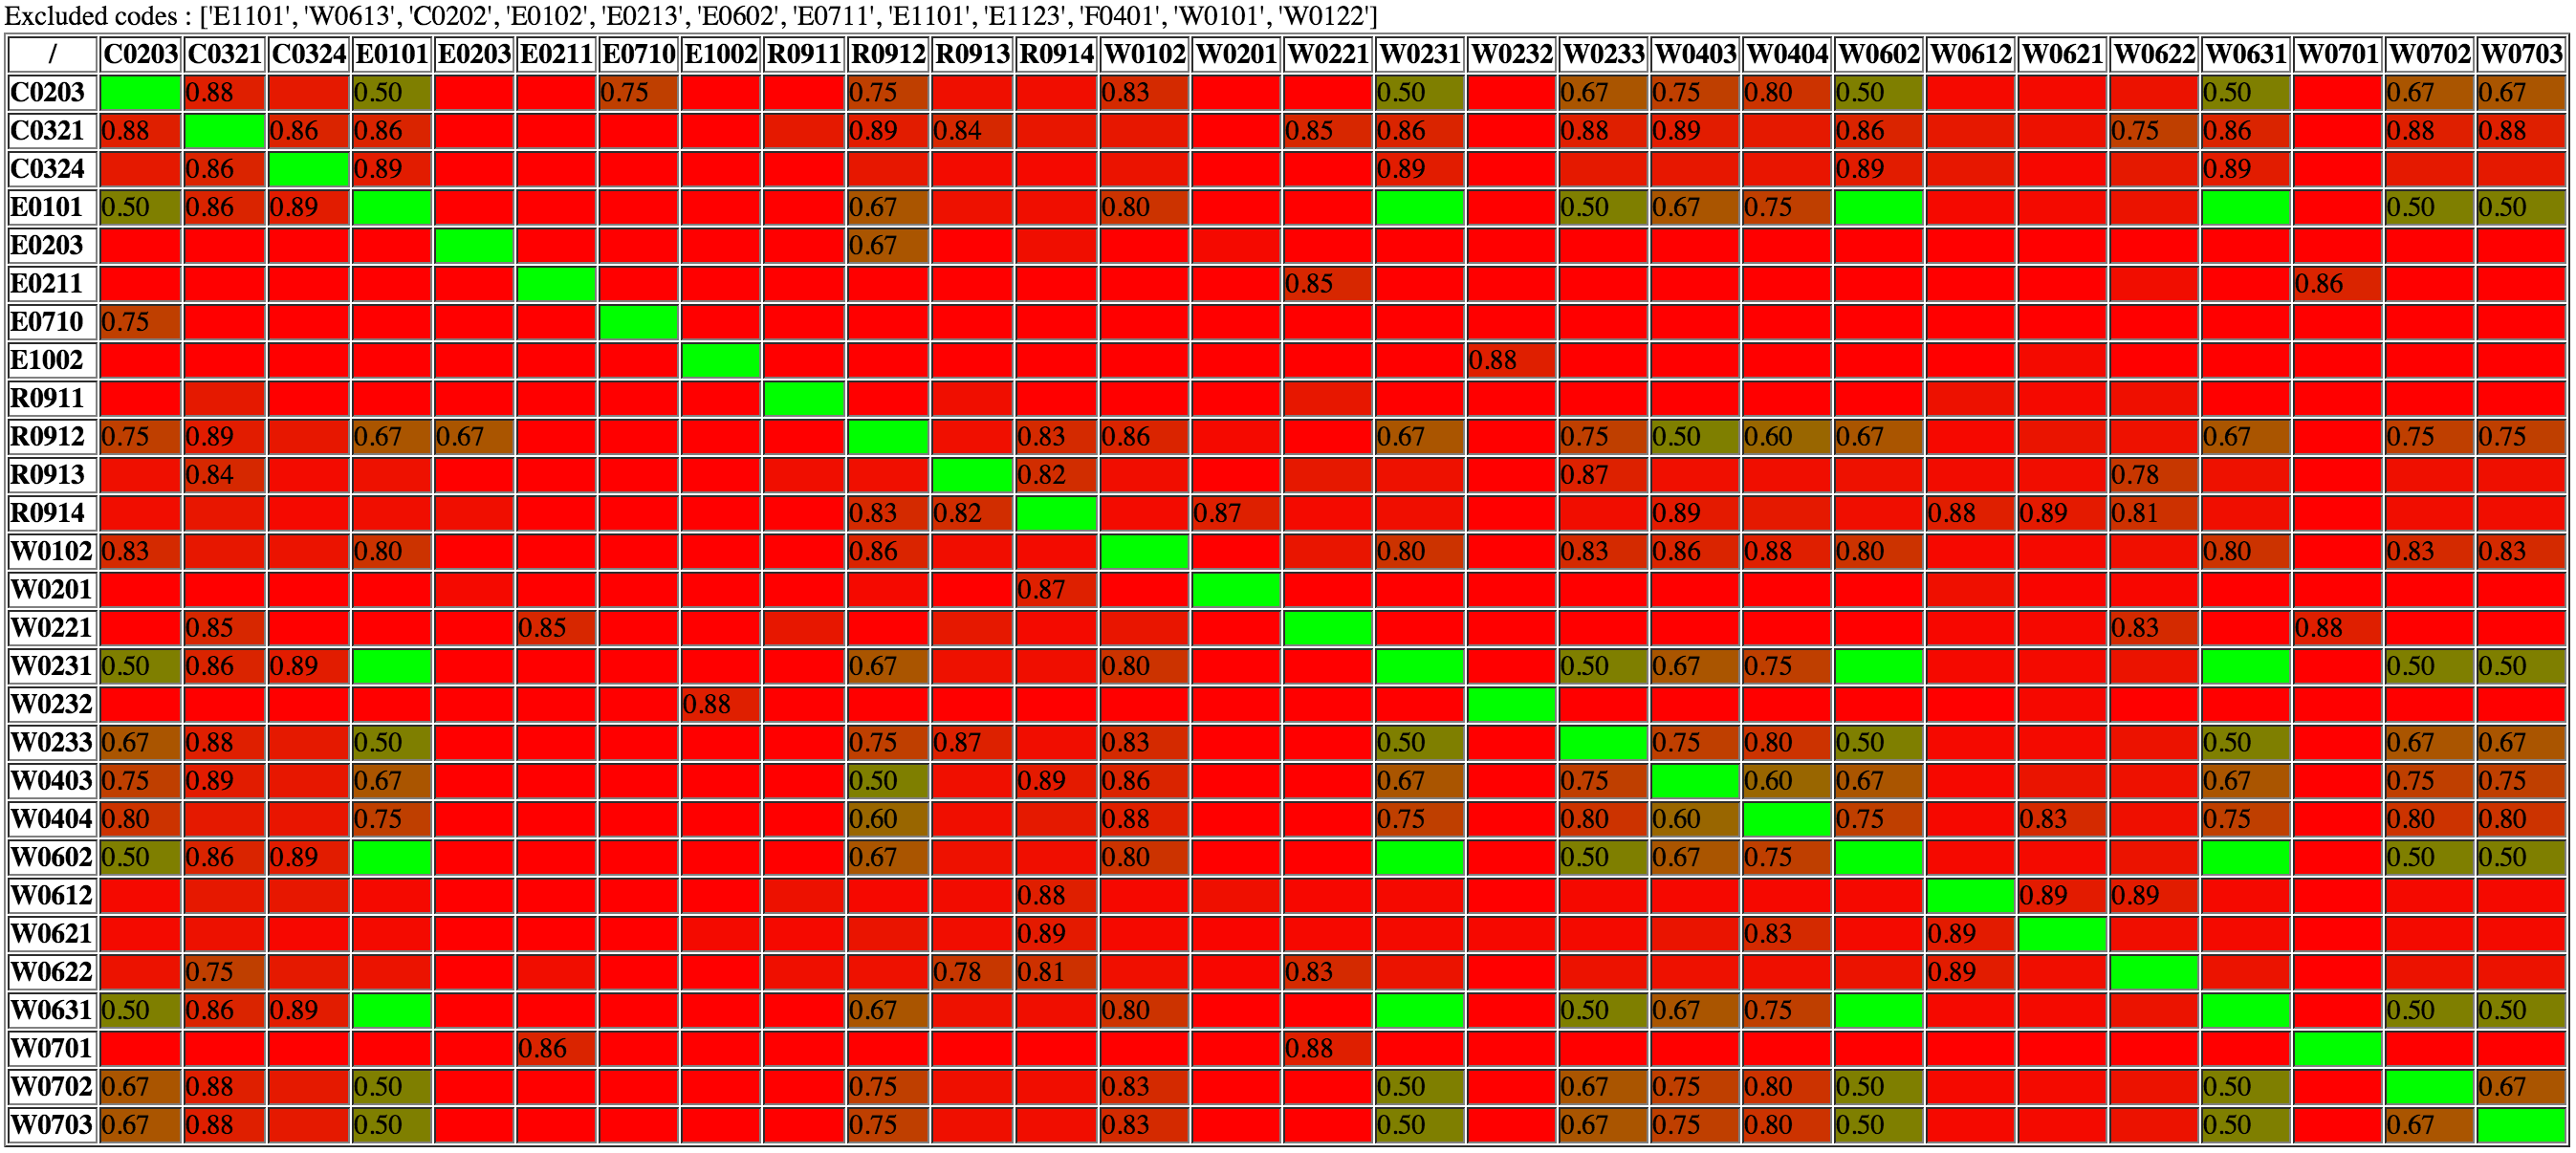
\includegraphics[angle=90,origin=c,totalheight=0.99\textheight]{cap1}

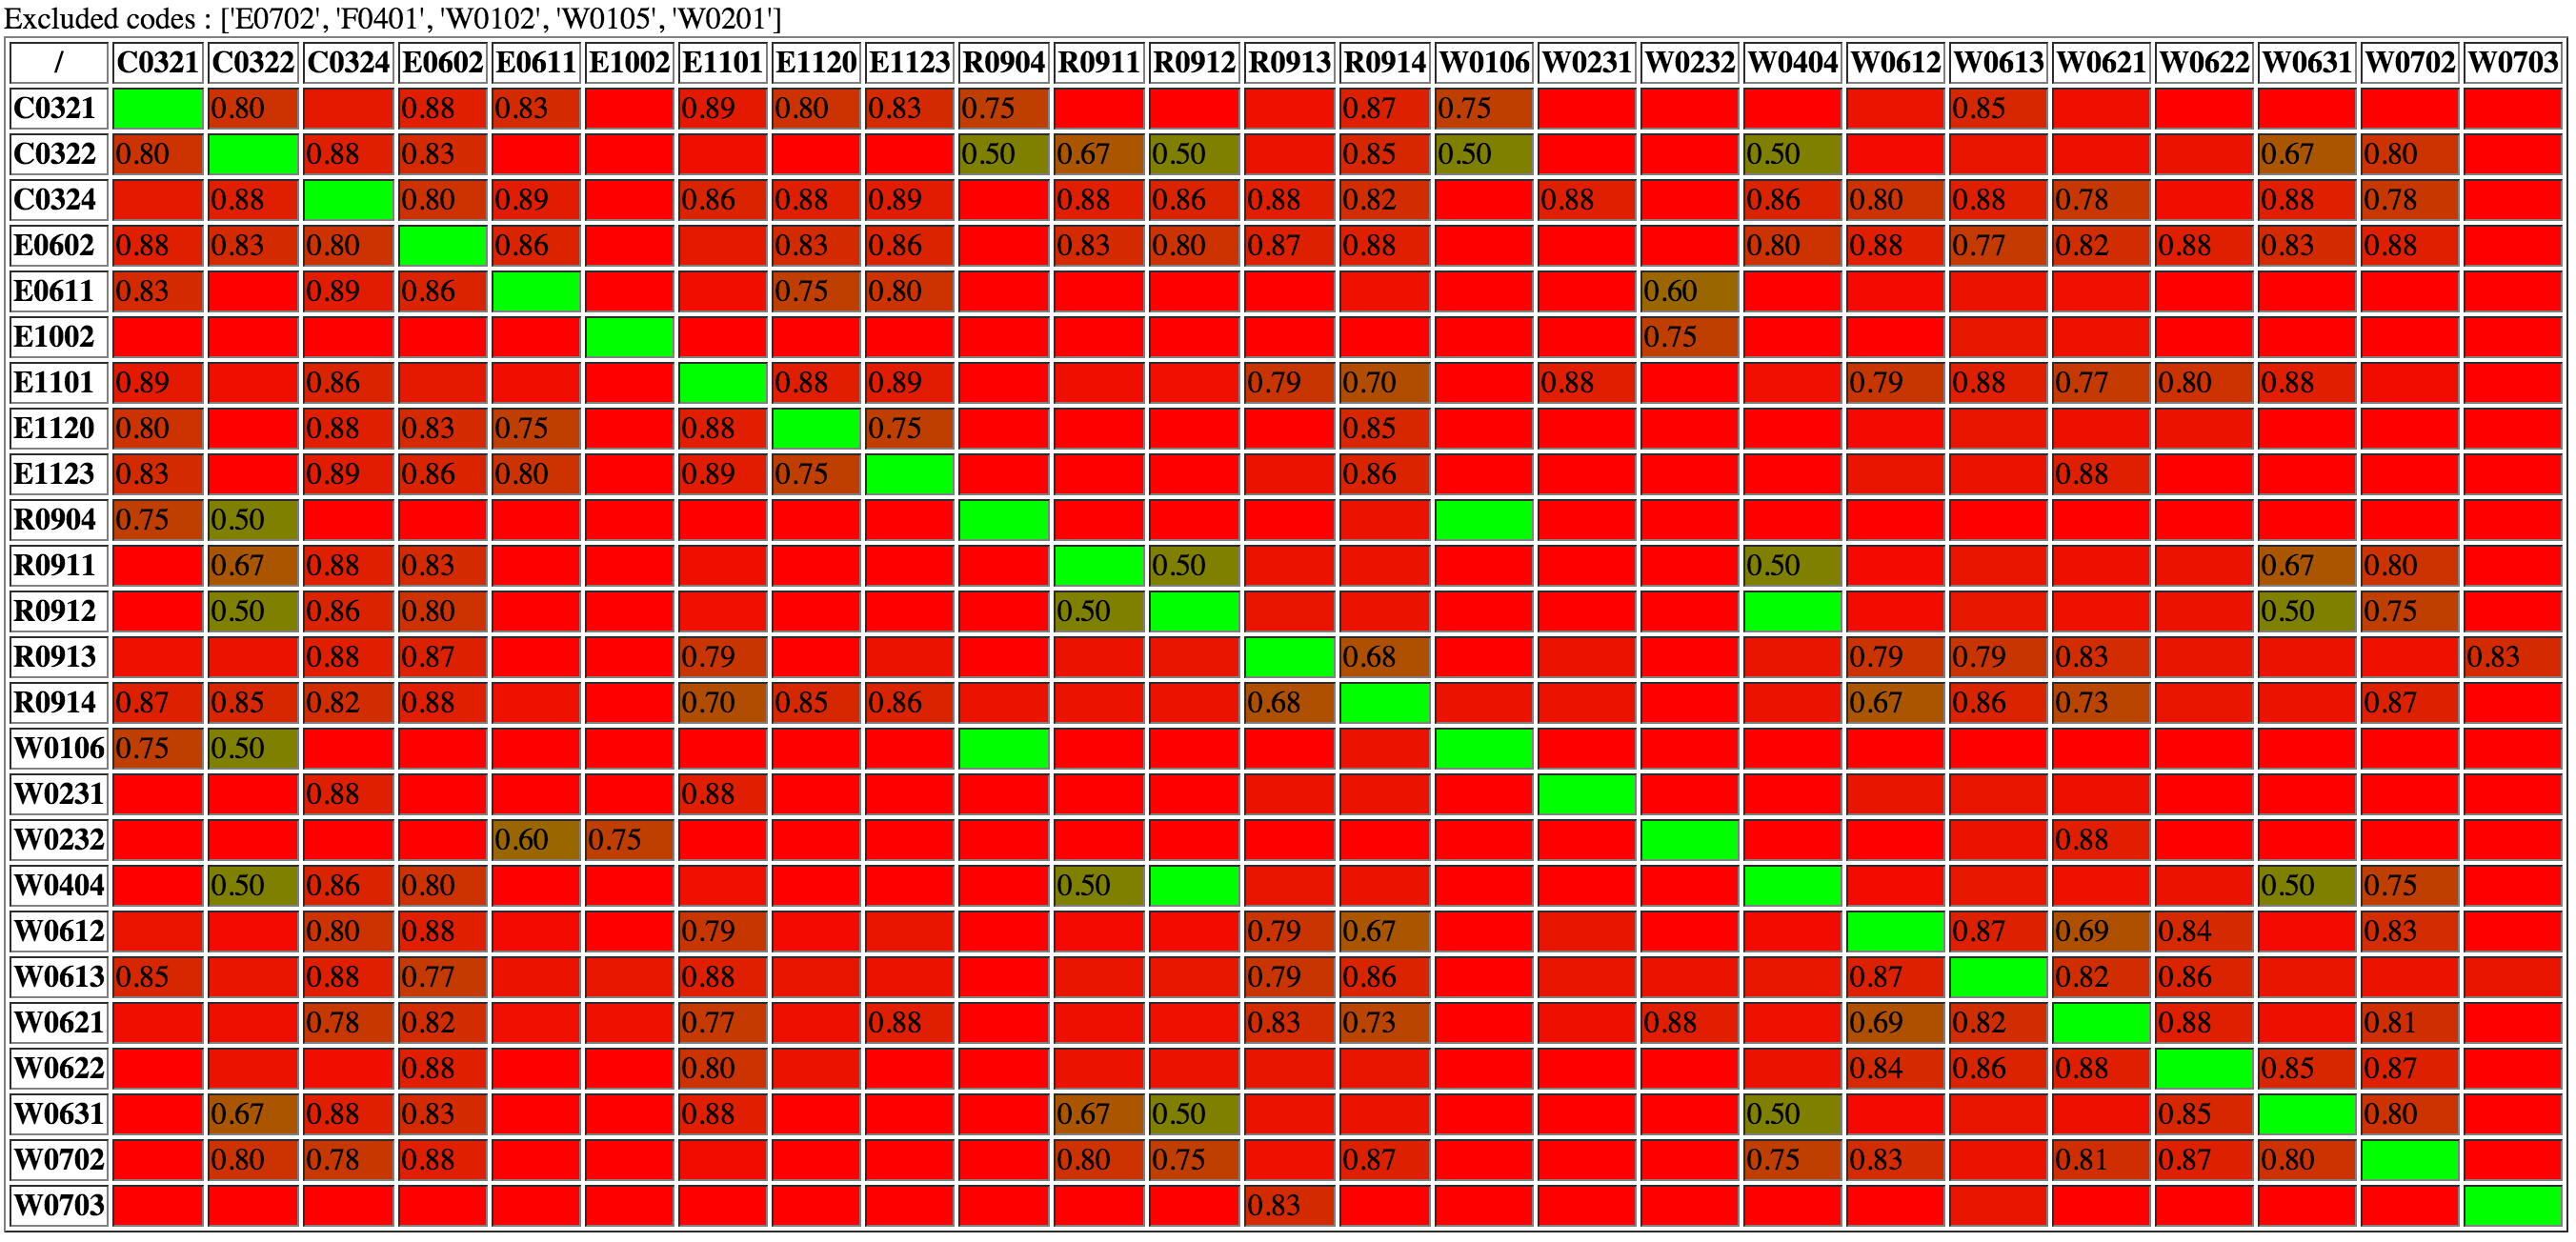
\includegraphics[angle=90,origin=c,totalheight=\textheight]{cap2}

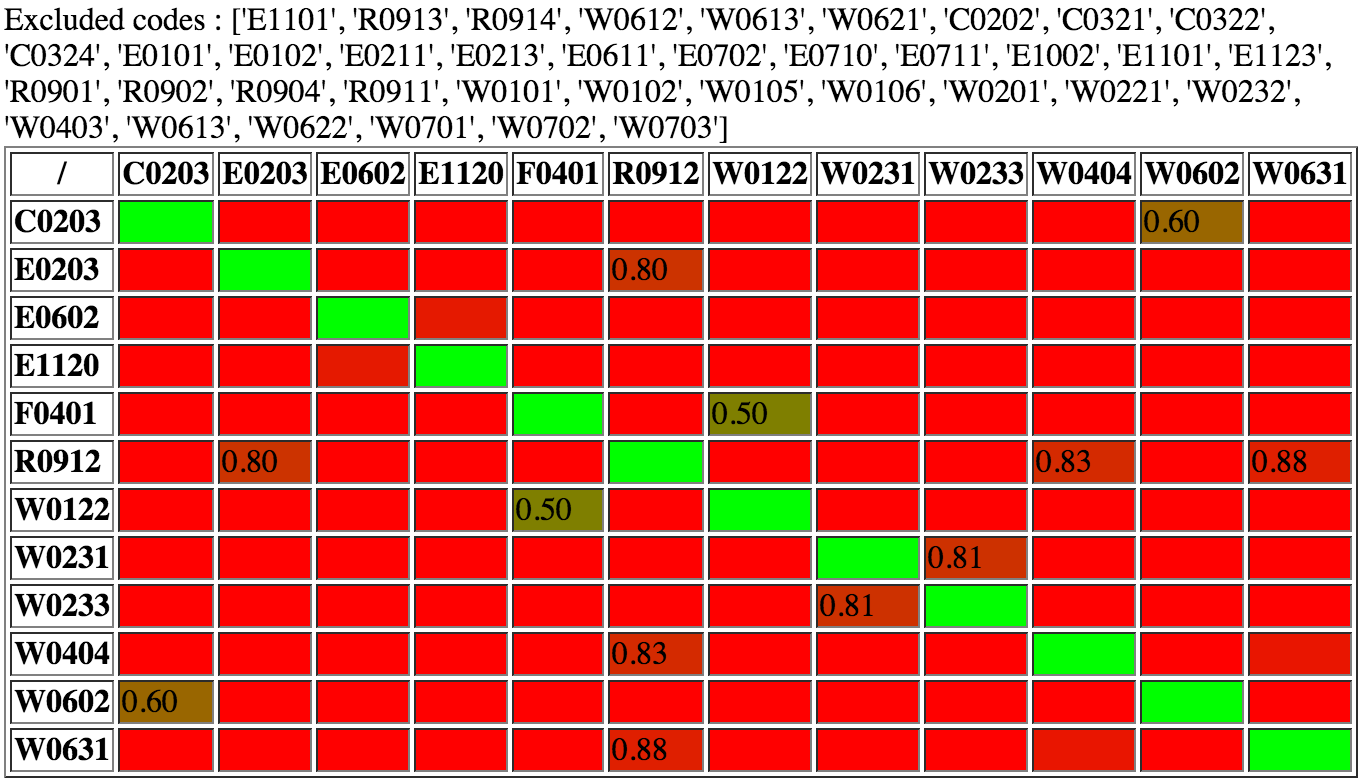
\includegraphics[angle=90,origin=c,totalheight=\textheight]{cap3}


\end{document}
